% =====================================================================
% EDA bölümü için ÖNERİLEN taslak metin. Otomatik üretildi: python scripts/run_eda.py
% Bütün sayılar kodun çıktısından geliyor. Kendi cümlelerinle uyarlayıp ara_rapor.tex'e ekle.
% Şekil yolları reports/ klasörüne göre (../figures/...). Overleaf'te klasör yapısına göre düzelt.
% 6 sayfa sınırı için ana metne 5-6 şekil yeter; isteğe bağlı şekiller yorum satırı olarak duruyor.
% =====================================================================

% ---------------------------------------------------------------------
% 1) ÖZET (abstract) içindeki \todo{EDA bulgularının 1--2 cümlelik özeti.} yerine öneri:
% ---------------------------------------------------------------------
% EDA, Golub verisinde sınıf bilgisi kullanılmadan PCA'nın ALL ve AML'yi ayırdığını, eğitim setinde 602 genin FDR düzeltmesi sonrası anlamlı olduğunu ve bu genlerin \%86'sının bağımsız MILE verisinde de aynı yönde farklılaştığını göstermiştir; buna karşın iki platform arasındaki ölçek farkı, veri setine özgü normalizasyonu zorunlu kılmaktadır.

% ---------------------------------------------------------------------
% 2) Bölüm III-D "Seçim Gerekçesi ve Uyumluluk" için öneriler
% ---------------------------------------------------------------------
% "Ortak gen sayısı: \todo{koddan}." yerine:
% Sembolü olmayan ve birden fazla gene eşlenen problar atıldıktan, aynı gene düşen problardan ortalama ifadesi en yüksek olan seçildikten sonra iki platformda 4.975 ortak gen kalmıştır.
% "İki sete aynı dönüşüm (kırpma ve log$_2$) uygulanacaktır." cümlesi EDA bulgusuyla çelişiyor. Yerine:
% Golub verisine kırpma (20--16.000) ve log$_2$ dönüşümü uygulanacaktır. MILE verisi ise GEO'da quantile normalize edilmiş ve 0--1 aralığına ölçeklenmiş olarak yayımlandığından bu dönüşüm ona uygulanmayacak; iki veri seti ortak genler üzerinde, her biri kendi içinde ölçeklenerek karşılaştırılacaktır.
% Tablo III, MILE satırları: $n$ = 1.292, AML = 542, Ölçek = Quantile normalize, 0--1, log benzeri.

% ---------------------------------------------------------------------
% 3) EDA BÖLÜMÜ
% ---------------------------------------------------------------------
\section{Keşifsel Veri Analizi (EDA)}
Bütün analizler Python ile yapılmış ve tek komutla (\texttt{python scripts/run\_eda.py}) yeniden üretilebilir. Golub test seti yalnızca betimleme ve batch karşılaştırması için kullanılmış; ayırt edici gen analizi yalnızca eğitim seti üzerinde yapılmıştır.

\subsection{Veri Kalitesi}
Golub etiketleri \texttt{actual.csv} dosyasından hasta numarasına göre eşlenmiş ve sınıf sayıları 27/11 (eğitim) ve 20/14 (test) olarak doğrulanmıştır. Test dosyasında hasta sütunları numara sırasında olmadığından, etiketler sütun sırasına göre atansaydı 34 test hastasının 14'ü yanlış etiketlenecekti. Veride eksik ya da sonsuz değer yoktur. Değerlerin \%28,67'si negatiftir (en küçük -28.400); negatif değerlerin \%99,28'i Affymetrix tarafından ``Absent'' olarak işaretlenmiştir, yani bu değerler arka plan çıkarımından kaynaklanan ölçüm gürültüsüdür. P/A/M çağrıları sınıf ve setler arasında benzerdir (``Present'' oranı \%25,6--\%29,7). 1.971 prob hiçbir hastada ``Present'' değildir; 58 AFFX kontrol probunun 34'ü de bu gruptadır.
% \begin{figure}[t]
% \centering
% 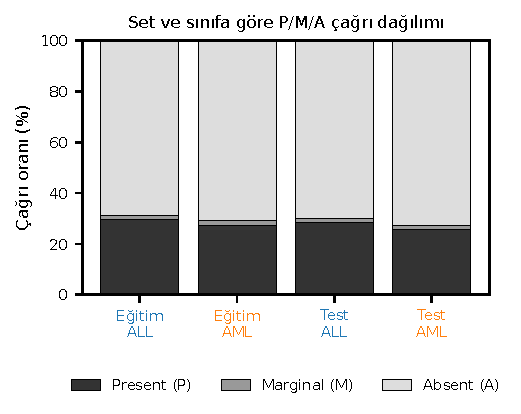
\includegraphics[width=\columnwidth]{../figures/fig02_pma_dagilimi.pdf}
% \caption{Set ve sınıfa göre P/M/A çağrı dağılımı.}
% \label{fig:pma}
% \end{figure}

\subsection{Betimsel İstatistikler ve Dönüşüm}
Ham ifade değerleri aşırı sağa çarpıktır (çarpıklık 7,08). Dudoit ve ark.~\cite{dudoit2002} izlenerek değerler 20--16.000 aralığına kırpılmış ve log$_2$ dönüşümü uygulanmıştır; çarpıklık 0,55'e inmiştir (Şekil~\ref{fig:dagilim}). Değerlerin \%32,72'si alt sınıra kırpılmaktadır. Dönüşümden sonra da hastalar arasında ölçek farkı sürmektedir: hasta medyanları 6,09--7,65 aralığında, en uç iki hastanın ortalamaları arasında yaklaşık 2,03 kat fark vardır. ALL ve AML ortalamaları neredeyse aynı olduğundan (6,965 ve 6,985) bu fark teknik kaynaklıdır.
\begin{figure}[t]
\centering
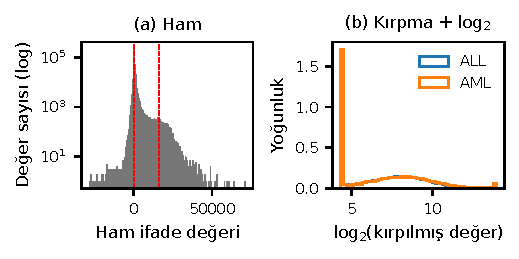
\includegraphics[width=\columnwidth]{../figures/fig03a_dagilim_ham_log.pdf}
\caption{(a) Ham ifade değerleri (kesikli çizgiler kırpma sınırları), (b) kırpma ve log$_2$ sonrası sınıf bazında dağılım.}
\label{fig:dagilim}
\end{figure}
% \begin{figure*}[t]
% \centering
% 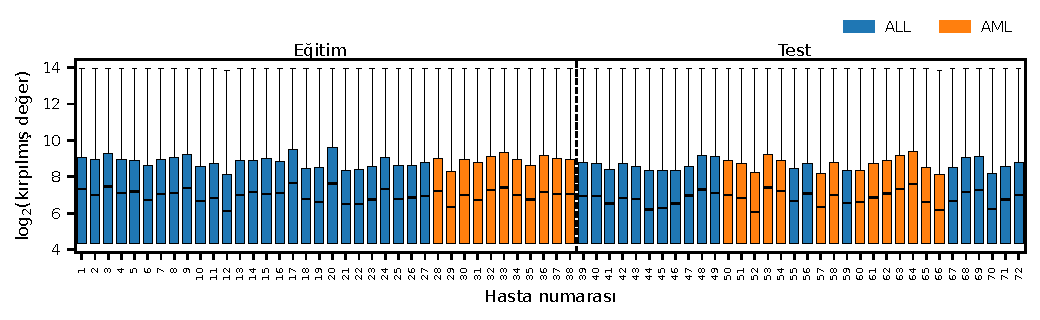
\includegraphics[width=\textwidth]{../figures/fig03b_ornek_kutu.pdf}
% \caption{Kırpma ve log$_2$ sonrası hasta bazında kutu grafiği.}
% \label{fig:kutu}
% \end{figure*}

\subsection{Boyut İndirgeme}
AFFX probları çıkarılmış 7.071 gen üzerinde yapılan PCA'da ilk iki bileşen varyansın \%17,67'sini açıklamaktadır; varyansın \%50'si için 13, \%90'ı için 54 bileşen gerekmektedir. Sınıf bilgisi kullanılmadığı halde PC1 ALL ve AML'yi ayırmaktadır (Mann--Whitney $1{,}8 \times 10^{-10}$; Şekil~\ref{fig:pca}), bu da Golub ve ark.~\cite{golub1999}'nin gözlemiyle uyumludur. Ancak ayrım kısmidir: sınıf siluet skoru PCA, t-SNE ve UMAP'te 0,27--0,30 aralığındadır. Eğitim ve test hastaları büyük ölçüde iç içedir (set siluet skoru 0,04--0,05).
\begin{figure}[t]
\centering
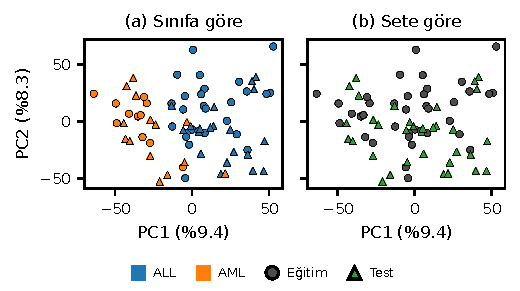
\includegraphics[width=\columnwidth]{../figures/fig04b_pca_pc1_pc2.pdf}
\caption{PC1--PC2 düzlemi: (a) sınıfa göre, (b) sete göre.}
\label{fig:pca}
\end{figure}
% \begin{figure}[t]
% \centering
% 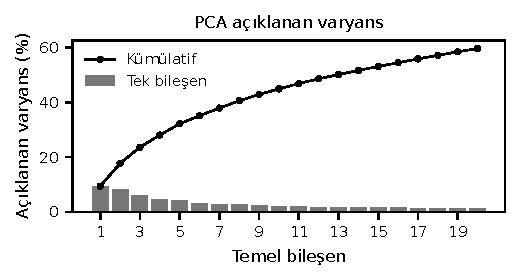
\includegraphics[width=\columnwidth]{../figures/fig04a_pca_varyans.pdf}
% \caption{PCA açıklanan varyans.}
% \label{fig:pcavar}
% \end{figure}
% \begin{figure}[t]
% \centering
% 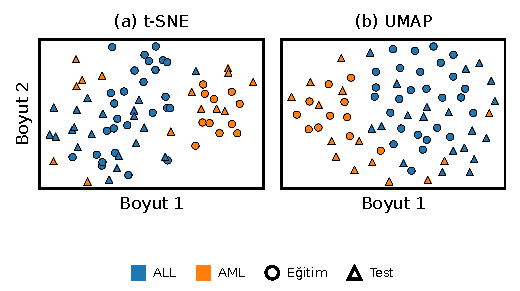
\includegraphics[width=\columnwidth]{../figures/fig04c_tsne_umap.pdf}
% \caption{t-SNE ve UMAP gömmeleri.}
% \label{fig:tsne}
% \end{figure}

\subsection{Ayırt Edici Genler}
Yalnızca eğitim setinde (38 hasta), iki sınıfta da sabit olan 476 gen çıkarıldıktan sonra kalan 6.595 gene Welch t-testi ve Benjamini--Hochberg FDR düzeltmesi uygulanmıştır. 602 gen $q<0{,}05$ ile anlamlıdır (274'ü AML'de, 328'i ALL'de yüksek); bunların 410'u en az iki kat fark göstermektedir. En anlamlı 50 genle yapılan hiyerarşik kümeleme hastaları sınıflarıyla yüksek uyumla ayırmaktadır (düzeltilmiş Rand indeksi 0,79; Şekil~\ref{fig:isi}). Listenin başında CST3, Zyxin, CD33 (AML) ve CD19, TCF3 (ALL) gibi soy belirteçleri yer almaktadır. Bu genler tüm eğitim seti üzerinde seçildiğinden kümeleme sonucu iyimserdir; modellemede gen seçimi çapraz doğrulama katları içinde yapılacaktır~\cite{ambroise2002}.
\begin{figure}[t]
\centering
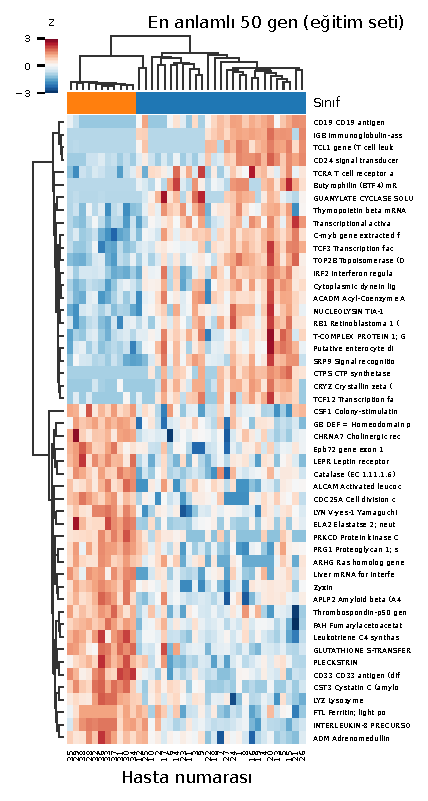
\includegraphics[width=\columnwidth]{../figures/fig05b_isi_haritasi_top50.pdf}
\caption{Eğitim setinde en anlamlı 50 genin z-skor ısı haritası ve hiyerarşik kümeleme.}
\label{fig:isi}
\end{figure}
% \begin{figure}[t]
% \centering
% 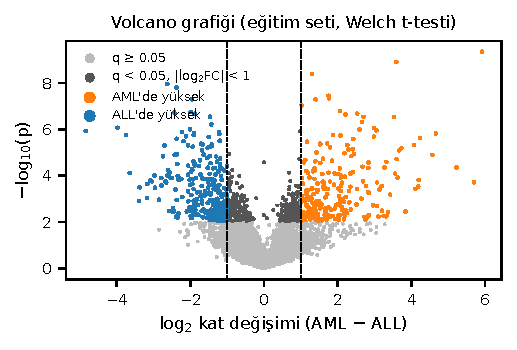
\includegraphics[width=\columnwidth]{../figures/fig05a_volcano.pdf}
% \caption{Volcano grafiği (eğitim seti).}
% \label{fig:volcano}
% \end{figure}

\subsection{Batch Analizi}
Test setinde AML oranı daha yüksek olduğundan (\%28,9 ve \%41,2) eğitim--test karşılaştırması yalnızca ALL hastaları arasında yapılmıştır. Test hastalarının genel ifade düzeyi her iki sınıfta da biraz daha düşüktür ve ALL hastalarının PCA'sında PC2 setleri ayırmaktadır (p = $4{,}3 \times 10^{-4}$). Gen bazında KS testinde 834 gen $p<0{,}05$ vermektedir (şans eseri beklenen 245), ancak FDR sonrası yalnızca 22 gen anlamlı kalmaktadır; her hasta kendi medyanına göre ortalandığında bu sayı 2'ye düşmektedir. Batch farkı zayıf, yaygın ve büyük ölçüde ölçek kaymasından kaynaklıdır.

Golub ve MILE ortak 4.975 gen üzerinde karşılaştırılmıştır. MILE 750 ALL ve 542 AML hastası içermekte ve quantile normalize edilmiş 0--1 ölçeğinde yayımlanmaktadır. Ham değerler doğrudan birleştirildiğinde PC1 varyansın \%97,2'sini açıklamakta ve yalnızca veri setini ayırmaktadır (veri seti siluet 0,99, sınıf siluet -0,00). Her gen kendi veri seti içinde z-skora çevrildiğinde veri seti farkı kaybolmakta, ALL/AML ayrımı ise iki veri setinde de aynı yönde ortaya çıkmaktadır (Şekil~\ref{fig:birlesik}). Golub eğitim setinde anlamlı bulunan genlerin \%86,0'ı MILE'da da aynı yönde farklıdır (tüm genlerde bu oran \%59,7); en anlamlı 50 genin 47'si tutarlıdır. Ters yönde çıkan genler (CDC25A, DYNLL1, UBE2V2) arasındaki CDC25A, Golub eğitim--test karşılaştırmasında da batch farkı gösteren tek ``en iyi 50'' genidir (Şekil~\ref{fig:yon}).
\begin{figure*}[t]
\centering
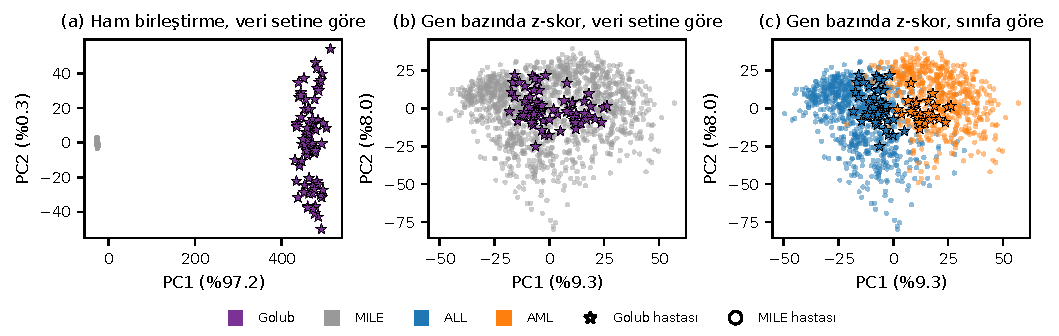
\includegraphics[width=\textwidth]{../figures/fig08b_birlesik_pca.pdf}
\caption{Golub ve MILE ortak genlerde birleşik PCA: (a) ham değerler, (b)--(c) gen bazında veri seti içi z-skor.}
\label{fig:birlesik}
\end{figure*}
\begin{figure}[t]
\centering
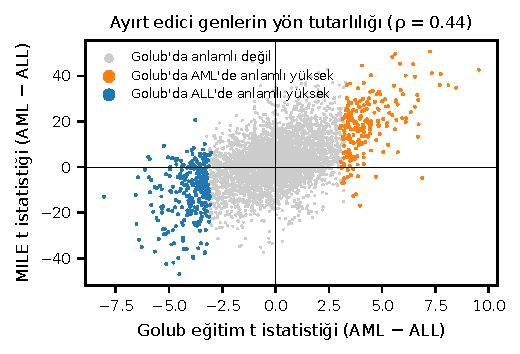
\includegraphics[width=\columnwidth]{../figures/fig08c_yon_tutarliligi.pdf}
\caption{Golub eğitim ve MILE t istatistikleri; renkli noktalar Golub'da anlamlı genler.}
\label{fig:yon}
\end{figure}
% \begin{figure}[t]
% \centering
% 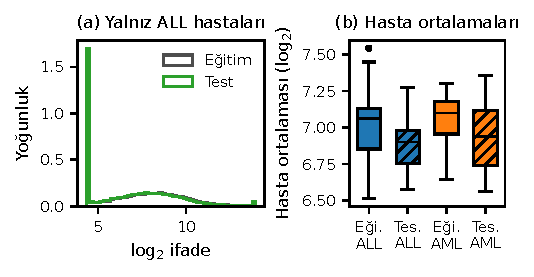
\includegraphics[width=\columnwidth]{../figures/fig06a_batch_dagilim.pdf}
% \caption{Golub eğitim--test karşılaştırması.}
% \label{fig:batch}
% \end{figure}
% \begin{figure}[t]
% \centering
% 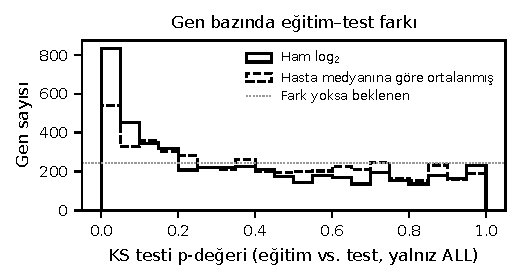
\includegraphics[width=\columnwidth]{../figures/fig06b_ks_pdegerleri.pdf}
% \caption{Gen bazında eğitim--test KS p-değerleri.}
% \label{fig:ks}
% \end{figure}
% \begin{figure}[t]
% \centering
% 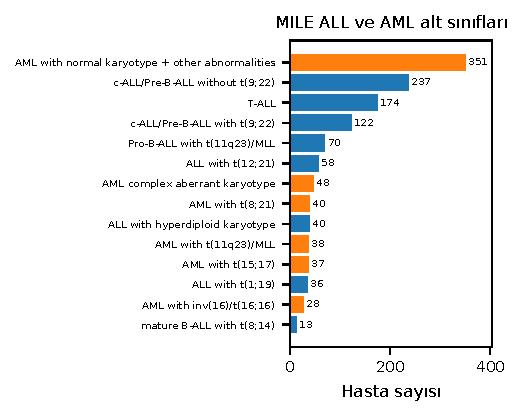
\includegraphics[width=\columnwidth]{../figures/fig07a_mile_alt_siniflar.pdf}
% \caption{MILE ALL ve AML alt sınıfları.}
% \label{fig:mile}
% \end{figure}
% \begin{figure}[t]
% \centering
% 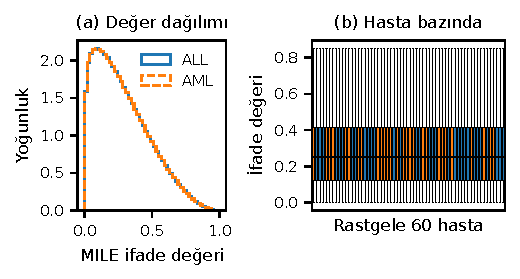
\includegraphics[width=\columnwidth]{../figures/fig07b_mile_olcek.pdf}
% \caption{MILE değer dağılımı ve hasta bazında kutu grafiği.}
% \label{fig:mileolcek}
% \end{figure}
% \begin{figure*}[t]
% \centering
% 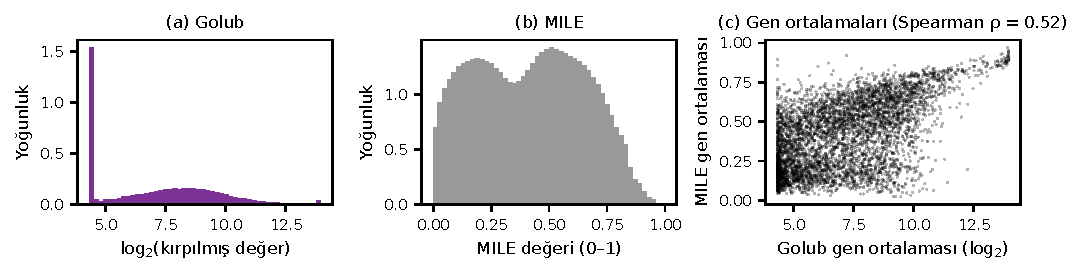
\includegraphics[width=\textwidth]{../figures/fig08a_golub_mile_olcek.pdf}
% \caption{Golub ve MILE ölçek karşılaştırması.}
% \label{fig:olcek}
% \end{figure*}

\subsection{Bulguların Özeti ve Modelleme İçin Çıkarımlar}
\begin{enumerate}[leftmargin=*]
  \item Golub etiketleri hasta numarasıyla eşlendi; sınıflar 27/11 (eğitim) ve 20/14 (test). Sütun sırasına göre eşleseydik testte 14 hasta yanlış etiketlenirdi. \textit{Çıkarım:} Etiketler her zaman hasta numarasıyla eşlenmeli; yükleyicideki assert kontrolleri korunmalı.
  \item Golub'da NaN/INF yok (0/0); değerlerin \%28,67'si negatif ve negatiflerin \%99,28'i 'Absent'. \textit{Çıkarım:} Modüldeki INF doldurma adımına bu veride gerek yok; negatifler ölçüm gürültüsü olduğu için alttan kırpılmalı.
  \item Ham değerler çok çarpık (çarpıklık 7,08); 20–16.000 kırpma + log2 sonrası 0,55. Değerlerin \%32,72'si alt sınıra yığılıyor. \textit{Çıkarım:} Kırpma + log2 Golub için standart ön işleme olmalı; her değere ayrı uygulandığı için sızıntı yaratmaz.
  \item 1.971 prob hiçbir hastada 'Present' değil; 58 AFFX kontrol probunun 34'ü de öyle. \textit{Çıkarım:} AFFX probları atılmalı; düşük ifade/varyans filtresi uygulanmalı ama yalnızca CV eğitim katlarında öğrenilmeli.
  \item Hasta ortalamaları arasında yaklaşık 2,03 kat fark var (log2 sonrası medyanlar 6,09–7,65); bu fark sınıfla ilişkili değil. \textit{Çıkarım:} Hasta bazında normalizasyon (ör. medyana göre ortalama) pipeline'da ablasyonla denenmeli.
  \item PCA'da sınıf bilgisi verilmeden PC1 ALL ile AML'yi ayırıyor (p = 1.8e-10); ancak PC1+PC2 varyansın yalnızca \%17,67'sini açıklıyor ve sınıf siluet skoru 0,29–0,30. \textit{Çıkarım:} Sınıf sinyali güçlü ama tek yöne sığmıyor; öznitelik seçimi ya da çok bileşenli doğrusal modeller uygun.
  \item Yalnız eğitim setinde 602 gen BH-FDR q < 0,05 ile anlamlı (410'u en az 2 kat farklı); en iyi 50 genle kümeleme sınıflarla ARI = 0,79 uyumlu. \textit{Çıkarım:} Az genle iyi ayrım mümkün; ama gen seçimi nested CV'nin her katında ayrı yapılmalı (seçim yanlılığı).
  \item Sınıf oranları dengesiz: Golub'da \%65,3 ALL; test setinde AML oranı eğitimden yüksek (eğitimde \%28,9, testte \%41,2). \textit{Çıkarım:} Stratified bölme, class\_weight ve dengeli doğruluk/ROC-AUC gibi dengesizliğe duyarlı metrikler kullanılmalı.
  \item Golub eğitim–test arasında hafif ama yaygın batch farkı: yalnız ALL'de 834 gen KS p < 0,05 (beklenen 245), FDR ile 22; hasta medyanına göre ortalayınca 2'ye iniyor. \textit{Çıkarım:} Batch farkının çoğu ölçek kayması; hasta bazında normalizasyon bunu büyük ölçüde gideriyor.
  \item MILE'da 750 ALL ve 542 AML var; veri quantile normalize, 0–1 ölçeğinde ve log benzeri (çarpıklık 0,70). Ortak gen sayısı 4.975. \textit{Çıkarım:} MILE'a kırpma + log2 uygulanmamalı; iki veri seti ortak genler üzerinden, her biri kendi içinde ölçeklenerek kullanılmalı.
  \item Ham birleştirmede veri seti farkı her şeyi bastırıyor (veri seti siluet 0,99, sınıf -0,00); gen bazında z-skor sonrası sınıf siluet 0,35, veri seti -0,18. \textit{Çıkarım:} Golub'da eğitilen model MILE'a uygulanacaksa genler her veri setinde ayrı ölçeklenmeli.
  \item Golub eğitimde anlamlı genlerin \%86,0'ı MILE'da da aynı yönde farklı; en iyi 50 genin 47'si tutarlı. Ters çıkanlar: CDC25A, DYNLL1, UBE2V2. \textit{Çıkarım:} Golub'da seçilen genler platformlar arası büyük ölçüde geçerli (AS2 için olumlu işaret); tutarsız genler yorumlanabilirlik bölümünde tartışılmalı.
\end{enumerate}
